\section{Allgemein}
\label{sec:RealAllgemein}
Die Realisation des Projekts CKI zeichnet sich durch die Implementierung eines modularen neuronalen Netzwerks aus, das für Aufgaben wie die Erkennung handschriftlicher Ziffern konzipiert wurde. Zum Einsatz kamen dabei Standard-C++-Technologien sowie eine CMake-basierte Projektstruktur für das Build-Management. Die Kernstruktur besteht aus Klassen für Neuron, Layer, und Network, die die Basis des Netzwerks bilden, ergänzt durch eine Util-Klasse für Hilfsfunktionen, wie Aktivierungsfunktionen und Datenverarbeitung.
Zusätzlich gibt es im Ordner „Test“ Unit-Tests mit den entsprechenden Attrappen für die MNIST-Datensätze. Die Unit-Tests sind mit Google-Tests implementiert.

\section{Abhängigkeiten}
\label{sec:RealAbhängigkeiten}
Das Projekt CKI kommt mit nur wenigen Abhängigkeiten aus.
Die, die es dennoch gibt, sind umso wichtiger für das erfolgreiche Ausführen der Applikation.
\\
Abhängigkeiten:
\begin{enumerate}
	\item \textbf{googletest:} \\
	\textbf{Version (Tag):} v1.14.0 \\
	\textbf{Git:} \url{https://github.com/google/googletest} \\
	\textbf{Beschreibung:} GoogleTest ist ein C++-Framework für Unit-Tests, das Assertions für die Überprüfung von Code und Funktionen für die Organisation und Ausführung von Tests bietet.

	\item \textbf{nlohmann/json:} \\
	\textbf{Version (Tag):} v3.11.3 \\
	\textbf{Git:} \url{https://github.com/nlohmann/json} \\
	\textbf{Beschreibung:} Nlohmann/json ist eine moderne, header-only C++ Bibliothek für die Verarbeitung von JSON-Daten, die einfache Integration und intuitive Nutzung bietet.

	\item \textbf{wichtounet/mnist:} (nicht mehr in Verwendung)\\
	\textbf{Version (Commit):} 3b65c35 \\
	\textbf{Git:} \url{https://github.com/wichtounet/mnist} \\
	\textbf{Beschreibung:} Wichtounet/mnist ist ein einfacher C++-Reader für den MNIST-Datensatz, der es ermöglicht, Trainings- und Testbilder sowie Labels zu lesen und zu verwenden.

	\item \textbf{nothings/stb:}\\
	\textbf{Version (Commit):} 5736b15 \\
	\textbf{Git:} \url{https://github.com/nothings/stb} \\
	\textbf{Beschreibung:} STB ist eine Sammlung plattformübergreifender Header-Dateien für C, die umfassende Funktionen für Grafik, Audio und Textverarbeitung ohne externe Abhängigkeiten bereitstellt. 
\end{enumerate}

\section{Architektur}
\label{sec:RealArchitektur}
\subsection{Klassen}
\label{sec:RealKlassen}
\subsubsection{Klassendiagramm}
\label{sec:RealKlassendiagramm}
\begin{figure}[H]
	\centering
		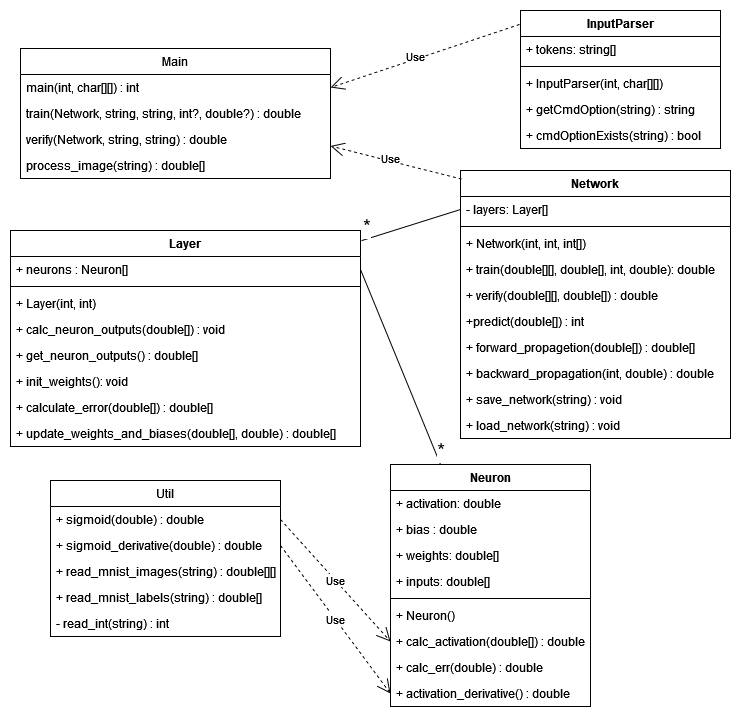
\includegraphics[width=1.00\textwidth]{klassendiagramm_after_implementation.png}
		\caption{Klassendiagramm nach der Realisation}
	\label{fig:klassendiagramm after implementation}
\end{figure}
Das ist das Klassendiagramm, wie die Applikation des Projektes CKI nach der Implementation aussieht. Somit sind die nötigen Anpassungen, die seit der Designphase zu treffen waren, ersichtlich.
\\
Wie zu sehen ist, gibt es etliche markante Änderungen in den Klassen Netzwerk und Layer. Dies kommt daher, dass in der Designphase aufgrund fehlendem oder unzureichendem Wissen die Struktur angepasst werden musste. Wie diese Klassen funktionieren sowie die wichtigsten Funktionen sind in den Abschnitten \ref{sec:RealKlassen}, bis \ref{sec:RealSnippetsCode} zu finden. 
\\
Interessant ist die Klasse InputParser, welche beim ursprünglichen Entwurf nicht anzutreffen war. Diese Klasse ist zuständig, einzelne Attribute aus dem Aufruf der CKI-Main-Funktion auszulesen und eine einfache Verwendung dieser zu gewährleisten. Dabei ist diese Klasse nicht selbst implementiert, sondern stammt von \url{https://stackoverflow.com/questions/865668/parsing-command-line-arguments-in-c}. Dementsprechend wird im weiteren Verlauf nicht weiter auf diese Funktion eingegangen.

\subsubsection{Netzwerk}
\label{sec:RealNetzwerk}
Die Network-Klasse repräsentiert das neuronale Netzwerk. Es unterstützt die Initialisierung des Netzwerks mit einer bestimmten Anzahl von Eingabe- und Ausgabeneuronen sowie eine variable Anzahl von versteckten Schichten und deren Grössen. Die Klasse bietet Funktionen für das Training des Netzwerks mit gegebenen Eingaben und Zielwerten, die Überprüfung der Netzwerkleistung und Vorhersagen für neue Eingaben. Dies ist möglich wegen der Durchführung von Vorwärts- und Rückwärtspropagation, die wichtigsten Algorithmen im Bereich des maschinellen Lernens (Mehr dazu unter Algorithmen \ref{sec:RealAlgorithmen}).
\\
Zusätzlich existieren noch zwei Funktionen in der Klasse, welche zuständig sind für die Speicherung und das Laden des Netzwerks in bzw. aus einer Datei.

\subsubsection{Layer}
\label{sec:RealLayer}
Die Layer-Klasse definiert die Layer im neuronalen Netzwerk, bestehend aus mehreren Neuronen. Sie bietet Funktionen zum Initialisieren und Setzen von Gewichten, Berechnen der Ausgaben der Neuronen basierend auf Eingaben, Berechnen der Fehler im Vergleich zu den Zielwerten und der Aktualisierung von Gewichten und Biases auf Basis von Fehlern und Lernrate.Jedes Layer-Objekt enthält eine Liste von Neuron-Objekten, die die Neuronen in diesem Layer repräsentieren. 

\subsubsection{Neuron}
\label{sec:RealNeuron}
Die Neuron-Klasse stellt ein einzelnes Neuron dar, inklusive seiner Gewichte, 
Bias, Eingaben, Aktivierungsfunktion und Summe der gewichteten Eingaben. Sie bietet Funktionen zur Berechnung der Aktivierung basierend auf den Eingaben, der Ableitung der Aktivierungsfunktion, der Fehlerberechnung im Vergleich zu einem Zielwert, sowie zur Speicherung der Gewichte und des Biases.
\\
Zur Berechnung der Aktivierung und deren Ableitung werden die statischen Utility-Funktionen Sigmoid und die Ableitung von Sigmoid aus der Utility-Klasse genutzt (Siehe auch \ref{sec:RealSigmoidAbleitungCode}).

\subsubsection{Utility}
\label{sec:RealUtility}
Die Util-Klasse bietet statische Hilfsfunktionen für das neuronale Netzwerk, darunter die Sigmoid-Aktivierungsfunktion und ihre Ableitung sowie Funktionen zum Lesen von MNIST-Bilddaten und Labels aus Dateien. Diese Hilfsfunktionen sind essenziell für die Vorverarbeitung von Eingabedaten und die Implementierung der Lernmechanismen im Netzwerk. 

\subsection{Ordnerstruktur}
\label{sec:RealOrdnerstruktur}
Im Kern des Projekts stehen die Hauptdateien, welche die essenziellen Klassen wie Neuron, Layer, Network und Util enthalten. Diese sind grundlegend für die Funktionalität des neuronalen Netzwerks. Die CMakeLists.txt unterstützt das Build-Management, vereinfacht die Kompilierung und Konfiguration. Der .gitignore sorgt dafür, dass unnötige Dateien und Ordner nicht in die Versionskontrolle einfliessen. Ein speziell dafür vorgesehener Test-Ordner beinhaltet Tests zur Überprüfung der Funktionalität, was die Zuverlässigkeit des Systems sicherstellt. Zusätzlich runden Dummy-Files und ein eigener Ordner für die MNIST-Datasets das Projekt ab, indem sie das Vorhandensein der Datensets für Training und Tests des Netzwerks garantieren.
\\
Das CKI-Projekt ist strukturiert in:
\begin{itemize}
	\item \textbf{Hauptdateien:} (kein Ordner, Rootverzeichnis) 
	Enthalten die Klassen Neuron, Layer, Network, und Util für die Kernlogik des neuronalen Netzwerks.
  \item \textbf{CMakeLists.txt:} (Im Rootverzeichnis)
	Für das Build-Management erleichtert das Kompilieren und die Konfiguration des Projekts.
  \item \textbf{.gitignore:} (Im Rootverzeichnis)
	Definiert Dateien und Ordner, die von Git-Versionierung ausgeschlossen sind, wie Build-Artefakte und IDE-spezifische Dateien.
  \item \textbf{Test-Ordner:} 
	Beinhaltet Testfälle zur Überprüfung der Funktionalität einzelner Komponenten und des Gesamtsystems.
	
	\begin{itemize}
		\item \textbf{Dummy-Files:} 
		Zusätzliche Dateien für Testzwecke. 
		\item \textbf{Unittests:}
		Tests zur Sicherstellung korrekter Funktionalität, Isolation von Fehlern. 
	\end{itemize}
	\item \textbf{MNIST-Datasets Ordner:} 
	Speichert die Datensätze für das Training und Testen des Netzwerks, insbesondere für die Erkennung handschriftlicher Ziffern.
\end{itemize}

\section{Code}
\label{sec:RealCode}
\subsection{Konzept}
Das Projekt CKI nutzt grundlegende Konzepte des maschinellen Lernens wie Vorwärts- und Rückwärts-Propagierung, Aktivierungsfunktionen (hier Sigmoid) und die Anpassung von Gewichten während des Trainingsprozesses. Die modulare Struktur, unterteilt in Schichten, Neuronen und Hilfsfunktionen, sowie die reine objektorientierte Implementation in C++ ohne externe Bibliotheken, abgesehen von Bibliotheken für Tests und Datenhandling, zeichnen die Architektur der Applikation aus.
\\
Um mehr über die hier erwähnten Funktionen zu erfahren, ist der Abschnitt \ref{sec:RealAlgorithmen} zu konsultieren.

\subsection{Algorithmen}
\label{sec:RealAlgorithmen}
\subsubsection{ Forward-Propagation}
\label{sec:RealForwardPropagation}
Die Forward-Propagation ist ein grundlegender Prozess in neuronalen Netzwerken, der es ermöglicht, Vorhersagen auf Basis von Eingabedaten zu treffen. Dabei werden die Eingabedaten durch das Netzwerk von der Eingabeschicht über eine oder mehrere versteckte Schichten bis zur Ausgabeschicht vorwärts geleitet. Jede Schicht besteht aus Neuronen, die über Gewichte mit den Neuronen der vorherigen Schicht verbunden sind. Die Daten werden in jedem Neuron durch eine Summationsfunktion verarbeitet, die die gewichteten Eingaben aufsummiert und einen Bias-Wert hinzufügt hat. Das Ergebnis dieser Summation wird dann durch eine Aktivierungsfunktion geleitet, um die Ausgabe des Neurons zu bestimmen.
\\
Die Aktivierungsfunktion bestimmt, wie Neuronen ihre Eingaben in Ausgaben umwandeln und ist entscheidend für die Fähigkeit des Netzwerks, komplexe Muster in den Daten zu erkennen. Beliebte Aktivierungsfunktionen sind die Sigmoid-, Tanh- und ReLU-Funktion.\footnote{vgl. Li \& Johnson \& Yeung, 2017; databasecamp, 2023}
\\
Sobald die Eingabedaten durch das Netzwerk propagiert worden sind und die Ausgabeschicht erreicht haben, wird das Ergebnis mit dem tatsächlichen Wert verglichen, um den Fehler der Vorhersage zu bestimmen. Dieser Fehler wird dann in einem separaten Prozess, der als Backpropagation bekannt ist, verwendet, um die Gewichte im Netzwerk anzupassen und die Vorhersagegenauigkeit zu verbessern.\footnote{vgl. Nüesch, 2023;  3Blue1Brown, 2017;}
%TODO add Math
\subsubsection{Back-Propagation}
\label{sec:RealBackPropagation}
Die Backpropagation, kurz für „backward propagation of errors“, ist ein Schlüsselmechanismus im Training neuronaler Netzwerke. Dieser Algorithmus ermöglicht es, die Gewichte des Netzwerks so anzupassen, dass der Gesamtfehler bei der Vorhersage minimiert wird. Backpropagation wird nach der Forward-Propagation angewendet, nachdem eine Vorhersage durch das Netzwerk gemacht und der Fehler zwischen der Vorhersage und dem tatsächlichen Wert berechnet wurde.
\\
Der Prozess der Backpropagation besteht aus zwei Hauptphasen: der Berechnung des Gradienten des Fehlers bezüglich aller Gewichte im Netzwerk und der anschliessenden Anpassung dieser Gewichte in die Richtung, die den Fehler minimiert. Der Gradient gibt an, in welche Richtung die Gewichte verändert werden müssen, um den Fehler zu verringern, und die Grösse der Anpassung wird durch die Lernrate bestimmt.
\\
Backpropagation nutzt die Kettenregel der Differenzialrechnung, um die Fehlergradienten für die Gewichte jeder Schicht vom Ausgang zurück zum Eingang effizient zu berechnen. Der berechnete Fehlergradient für jede Gewichtung zeigt, wie eine kleine Änderung in diesem Gewicht den Gesamtfehler beeinflusst. Durch die systematische Anpassung der Gewichte basierend auf diesen Gradienten kann das Netzwerk schrittweise verbessert werden, um genauere Vorhersagen zu liefern.
\\
Insgesamt ermöglicht Backpropagation das effiziente Training tiefer neuronaler Netzwerke, indem es systematisch die Netzwerkgewichte anpasst, um den Fehler zwischen den Vorhersagen des Netzwerks und den tatsächlichen Werten zu minimieren, was zu einer verbesserten Modellleistung führt.\footnote{vgl. Nüesch, 2023; 3Blue1Brown, 2017; Karpathy, 2016; Roy, 2022; Li \& Johnson \& Yeung, 2017; }
%TODO add Math
\subsection{Schlüsselpassagen \& Snippets}
\label{sec:RealSnippetsCode}
Die wichtigsten Funktionen in einem neuronalen Netzwerk sind die beiden Propagation, vorwärts als auch rückwärts. Wobei diese das Grundgerüst für die drei Hauptfunktionen, Train, Verify \& Predict bilden.

\subsubsection{Train}
\label{sec:RealTrainCode}
\begin{lstlisting}[language=C++]
double Network::train(std::vector<std::vector<double>> &inputs, std::vector<double> &labels, int epochs, double learning_rate){
    double total_error = 0;
    for(int epoch = 0; epoch<epochs; epoch++ ){
        for(std::size_t i = 0; i < inputs.size(); i++){
            std::vector<double> outputs = Network::forward_propagation(inputs[i]);
            total_error += Network::backward_propagation(labels[i], learning_rate);
            total_error /= 2;
        }
    }
    return total_error;
}

\end{lstlisting}
\addcontentsline{lol}{lstlisting}{\protect\numberline{\thelstlisting} Train Funktion aus der Netzwerk-Klasse}
Die Funktion, welche für das Lernen des neuronalen Netzwerks verantwortlich ist, ist simpel aufgebaut. Sie erhält primär zwei Listen: eine Liste aus Bildern und eine Liste aus Beschriftungen für die Bilder. Danach nutzt Train die Funktionen der Forward- und Back-Propagation, um zuerst das Bild durch das Netzwerk bewerten zulassen und dann diese Bewertung mithilfe der Beschriftungen zu korrigieren. Dies tut sie für den gesamten Datensatz oder durch eine zukünftige Erweiterung in einzelnen Blöcken (für höhere Effektivität) und der Anzahl Epochen entsprechend.

\subsubsection{Verify}
\label{sec:RealVerifyCode}
\begin{lstlisting}[language=C++]
double Network::verify(const std::vector<std::vector<double>> &inputs, const std::vector<double> &labels){
    int correct = 0;
    for (std::size_t i = 0; i < inputs.size(); ++i){
        if (Network::predict(std::vector<double>(inputs[i])) == static_cast<int>(labels[i])){
            correct++;
        }
    }
    return static_cast<double>(correct) / static_cast<double>(inputs.size());
}
\end{lstlisting}
\addcontentsline{lol}{lstlisting}{\protect\numberline{\thelstlisting} Verify Funktion aus der Netzwerk-Klasse}
Die Funktion ist eigentlich gleich aufgebaut wie „Train“, jedoch mit dem markanten Unterschied, dass keine Back-Propagation zum Einsatz kommt. So werden die Bewertungen des neuronalen Netzwerks nur als richtig oder falsch bewertet und nicht korrigiert.

\subsubsection{Predict}
\label{sec:RealPredictCode}
\begin{lstlisting}[language=C++]
int Network::predict(const std::vector<double> &input){
    std::vector<double> outputs = Network::forward_propagation(input);
    return static_cast<int>(std::distance(outputs.begin(), std::max_element(outputs.begin(), outputs.end())));
}
\end{lstlisting}
\addcontentsline{lol}{lstlisting}{\protect\numberline{\thelstlisting} Predict Funktion aus der Netzwerk-Klasse}
Diese Funktion erhält nur ein einziges Bild als Attribut. Dieses Bild wird durch die Forward-Propagation bewertet. Die Bewertung wiederum besteht nur aus einer Liste von zehn Prozentzahlen (für die Ziffern von 0 bis 9) und damit diese besser für einen Menschen lesbar wird, muss die höchste Prozentzahl aus der Liste gesucht werden. Deren Index wird dann als errechnete Zahl zurückgegeben.
\\
(Diese Funktion ist ein Zusammenzug aus der Predic-Funktion und Logic aus der main.cpp-Datei.)

\subsubsection{Forward-Propagation}
\label{sec:RealForwardPropagationCode}
\begin{lstlisting}[language=C++]
std::vector<double> Network::forward_propagation(const std::vector<double>& input){
    layers[0].calc_neuron_outputs(input);

    for (int i = 1; i < layers.size(); ++i){
        std::vector<double> inputs = layers[i - 1].get_neuron_outputs();
        layers[i].calc_neuron_outputs(inputs);
    }

    return layers[layers.size()-1].get_neuron_outputs();
}
\end{lstlisting}
\addcontentsline{lol}{lstlisting}{\protect\numberline{\thelstlisting} Forward-Propagation Funktion aus der Netzwerk-Klasse}
In dieser Funktion wird eine Liste von grossen Fliesskommazahlen übernommen. Diese sind die einzelnen Pixel, in dem zu bearbeiteten Bild, welche nur einen Helligkeitswert beinhalten. Diese Pixel werden an den ersten Layer im Netzwerk übergeben. Dieser kalkuliert durch die Sigmoid-Funktion neue Ausgabewerte. Die Ausgabewerte werden mit der For-Schleife durch alle Schichten des Netzwerks weitergereicht, bis diese am Ende ausgelesen und als Rückgabewert dieser Funktion genutzt werden. Die Ausgabewerte haben zwar das gleiche Datenformat, unterscheiden sich jedoch anhand ihrer Grösse (Länge der Liste) und den tatsächlichen Werten.

\subsubsection{Back-Propagation}
\label{sec:RealBackPropagationCode}
\begin{lstlisting}[language=C++]
double Network::backward_propagation(const int& target, double learning_rate){
    std::vector<double> inputs (10, 0);
    inputs[target] = 1;
    std::vector<double> error = layers[layers.size()-1].calculate_error(inputs);

    double total_error = 0;
    for(double& e : error) { //remove for better performance
        total_error += e;
    }

    total_error/=error.size();

    //std::cout << total_error << std::endl;

    for (int i = layers.size() - 1; i >= 0; --i){
        error = layers[i].update_weights_and_biases(error, learning_rate);
    }
    return total_error;
}
\end{lstlisting}
\addcontentsline{lol}{lstlisting}{\protect\numberline{\thelstlisting} Backward-Propagation Funktion aus der Netzwerk-Klasse}
Im Gegensatz zur Forward-Propagation wird in der Back-Propagation ein Wert nicht von der ersten Schicht zur letzten übergeben, sondern Rückwerts von dem letzten Layer bis zur Eingabe zurück.
\\ 
Dabei muss zuerst die Abweichung von der erhaltenen Ausgabe (aus der Forward-Propagation) mit der erwarteten Ausgabe abgeglichen und der Fehler berechnet werden. Nun wird ähnlich zur Forward-Propagation dieser Fehler durch die einzelnen Schichten geschickt und dort verwendet, um die Gewichtungen und Biases für jedes Neuron anzupassen. Dies passiert in einer eigenen Funktion im Layer.

\subsubsection{Anpassung von Gewichtungen und Biases}
\label{sec:RealAnpassungVonGewichtungenUndBiasesCode}
\begin{lstlisting}[language=C++]
std::vector<double> Layer::update_weights_and_biases(const std::vector<double>& error, double learning_rate){
    std::vector<double> prev_layer_error(Layer::neurons[0].weights.size(), 0.0);

    for (size_t i = 0; i < Layer::neurons.size(); ++i){
        Neuron &neuron = Layer::neurons[i];
        const double neuron_error = error[i];
        const double activation_derivative = neuron.activation_derivative();

        for (size_t j = 0; j < neuron.weights.size(); ++j){
            prev_layer_error[j] += neuron.weights[j] * neuron_error;

            const double delta_weight = neuron_error * activation_derivative * neuron.inputs[j];
            neuron.weights[j] -= learning_rate * delta_weight;
        }
        neuron.bias += learning_rate * neuron_error * activation_derivative;
    }
    return prev_layer_error;
}
\end{lstlisting}
\addcontentsline{lol}{lstlisting}{\protect\numberline{\thelstlisting} Anpassung von Gewichtungen und Biases aus der Layer-Klasse}
Dies ist die Funktion, die in der Back-Propagation aufgerufen wird.
\\
Dabei wird für jedes Neuron für jede Gewichtung eine eigene Anpassung gesucht. Um dies zu erreichen, werden mehrere Werte benötigt: 
Der Fehler des Neurons, der Input des Neurons, die Ableitung der Aktivierung und die Learningrate.
Nun können die Änderungen bei der Gewichtung und dem Bias berechnet werden. Die Abweichung der Gewichtung ist ein Produkt des Inputs in diesem Neuron, dem Fehler, der Ableitung der Sigmoid-Funktion und der Learningrate. Die Korrektion für das Bias ist fast identisch zu der Abweichung der Gewichtung. Es ist ebenfalls ein Produkt der gleichen Faktoren, abgesehen von der Learningrate und dem Input.
\\
Zusätzlich kann der Fehler für den nächsten Layer berechnet werden. Dieser wird benötigt, um die Backpropagation auf den nächsten Layer auszudehnen und dort dieselben Schritte auszuführen. Dabei setzt sich der Fehler für den nächst oberen Layer zusammen, aus dem Fehler und dem entsprechenden Gewicht für das Neuron. Dabei wird der Fehler neu gewichtet und zusammen mit allen anderen neu-gewichteten Fehlern für dieses eine Neuron auf der nächsten Ebene aufsummiert.

\subsubsection{Sigmoid \& Ableitung}
\label{sec:RealSigmoidAbleitungCode}
\begin{lstlisting}[language=C++]
double Util::sigmoid(double x){
	return 1.0 / (1.0 + exp(-x));
}

double Util::sigmoid_derivative(double x){
	double s = sigmoid(x);
	return s * (1.0 - s);
}
\end{lstlisting}
\addcontentsline{lol}{lstlisting}{\protect\numberline{\thelstlisting} Sigmoid \& Ableitung aus der Util-Klasse}
Das sind die mathematischen Implementierungen der Sigmoid-Funktion und deren mathematischen Abweichungen. Diese Funktionen sind zuständig für die einzelnen Aktivierungen der Neuronen und verschieben eine Zahl in den Wertebereich zwischen 0 und 1.
\begin{figure}[H]
	\centering
		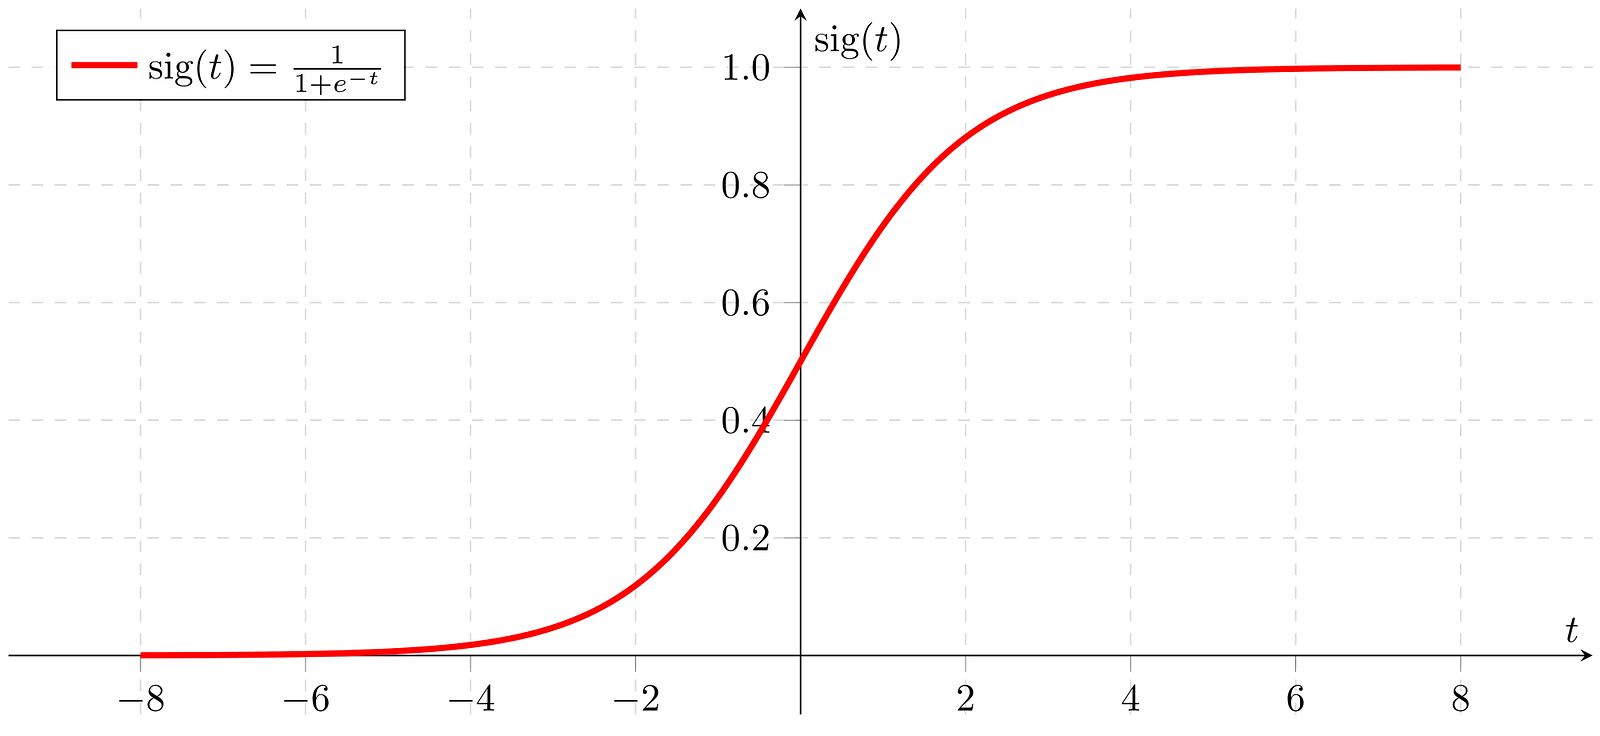
\includegraphics[width=0.75\linewidth]{sigmoid.png}
		\caption{Sigmoid Funktion}
	\label{fig:sigmoid}
\end{figure}

\subsubsection{MNIST-Reader}
\label{sec:RealMNISTReaderCode}
\begin{lstlisting}[language=C++]
std::vector<std::vector<double>> Util::read_mnist_images(const std::string &filename){
    std::ifstream file(filename, std::ios::binary);
    if (file.is_open()){
        int magic_number = read_int(file);
        int number_of_images = read_int(file);
        int number_of_rows = read_int(file);
        int number_of_columns = read_int(file);

        std::vector<std::vector<double>> images(number_of_images, std::vector<double>(number_of_rows * number_of_columns));

        for (int i = 0; i < number_of_images; ++i){
            for (int r = 0; r < number_of_rows * number_of_columns; ++r){
                unsigned char temp = 0;
                file.read(reinterpret_cast<char*>(&temp), sizeof(temp));
                images[i][r] = (double)temp / 255.0; // Normalizing pixel values to [0, 1]
            }
        }
        return images;
    }else{
        throw std::runtime_error("Cannot open file: " + filename);
    }
}
\end{lstlisting}
\addcontentsline{lol}{lstlisting}{\protect\numberline{\thelstlisting} MNIST-Reader aus der Util-Klasse}
Um die Daten aus den von \url{http://yann.lecun.com/exdb/mnist/} stammenden UByte-Dateien auszulesen, müssen gewisse Byte-Werte aus den Dateien ausgelesen werden. Die hier aufgeführte Funktion dient dazu Bilder aus diesen Dateien auszulesen und ist beispielhaft auch für die Labels.
\\
Die Implementierung ist nach dem Muster von \url{http://yann.lecun.com/exdb/mnist/} implementiert. So sind in den ersten vier Byte gespeichert, wie viele Bilder/Beschriftungen im Datensatz zu finden sind. Um dies auszulesen, ist in einer eigenen Funktion implementiert (read\_int). Nach den ersten vier Byte müssen die restlichen Bytes in eine Liste eingetragen, in eine ganze Zahl interpretiert (zwischen 0 und 255) und auf den Wert zwischen 0 und 1 gebracht werden. Man spricht auch von der Normalisierung der Pixel-Werte.

\subsubsection{Ersten 4 Bytes}
\label{sec:RealErsten4BytesCode}
Dies ist die oben angesprochene „read\_int“-Funktion.
\begin{lstlisting}[language=C++]
int Util::read_int(std::ifstream &file){
    unsigned char bytes[4];
    file.read(reinterpret_cast<char*>(bytes), sizeof(bytes));
    return (int)((bytes[0] << 24) | (bytes[1] << 16) | (bytes[2] << 8) | bytes[3]);
}
\end{lstlisting}
\addcontentsline{lol}{lstlisting}{\protect\numberline{\thelstlisting} Utility Funktion für den MNIST-Reader aus der Util-Klasse}
Die Funktion wurde mit der Hilfe von Stack Overflow unter dem Link \url{https://stackoverflow.com/questions/604431/c-reading-unsigned-char-from-file-stream} erstellt.
\\
Zuerst wird ein Array in der Grösse von vier Bytes erstellt und vier Bytes aus einer Datei eingelesen. Danach werden die vier Bytes zu einer einzigen ganzen Zahl zusammengesetzt. Dies geschieht, indem die Bytes um jeweils 8 Bits nach links verschoben werden und somit das erste Byte die acht höchsten Stellen der ganzen Zahl symbolisiert, danach das zweite Byte und so folgend die restlichen Bytes.

\subsubsection{Bild Vorverarbeitung}
\label{sec:RealBildVorverarbeitungCode}
\begin{lstlisting}[language=C++]
std::vector<double> process_image(const char* filename) {
    int width, height, channels;
    unsigned char* img = stbi_load(filename, &width, &height, &channels, 0);
    if (img == nullptr) {
        std::cerr << "Error in loading the image" << std::endl;
        exit(1);
    }

    unsigned char* resized_img = new unsigned char[28 * 28 * channels];
    stbir_resize_uint8(img, width, height, 0, resized_img, 28, 28, 0, channels);

    std::vector<double> image_data(28 * 28);
    for (int i = 0; i < 28 * 28; ++i) {
        int j = i * channels;
        double gray = 0.299 * resized_img[j] + 0.587 * resized_img[j + 1] + 0.114 * resized_img[j + 2];
        image_data[i] = gray / 255.0; // Normalize to [0, 1]
    }

    stbi_image_free(img);
    delete[] resized_img;

    return image_data;
}
\end{lstlisting}
\addcontentsline{lol}{lstlisting}{\protect\numberline{\thelstlisting} Bild Vorverarbeitung für Nutzer-gelieferte Bilder}
Dies Funktion lädt ein Bild von der angegebenen Datei, skaliert es auf 28x28 Pixel herunter und konvertiert es in Graustufen. Zuerst wird das Bild geladen, wobei Breite, Höhe und Kanäle des Bildes erfasst werden. Falls das Laden fehlschlägt, wird eine Fehlermeldung ausgegeben und das Programm beendet. Anschließend wird das Bild auf die Größe 28x28 Pixel verkleinert, wobei die Anzahl der Kanäle beibehalten wird. Danach wird für jeden Pixel ein Graustufenwert berechnet, indem eine gewichtete Summe seiner RGB-Werte gebildet und durch 255 geteilt wird, um den Wert auf den Bereich [0, 1] zu normalisieren. Diese Werte werden gespeichert und am Ende der Funktion zurückgegeben. Zum Schluss werden der Speicher des ursprünglichen und des skalierten Bildes freigegeben, um Speicherlecks zu verhindern.
\\
Diese Funktion wird verwendet, um in der Ausführung von Predict das Bild des Nutzers zu übernehmen und auf das geforderte Format zu verkleinern.